% !TEX root = main.tex
\section{The Earlier 72-Pair Validation Set: Results, Provenance, and Selection Bias}\label{app:validation-set-72}
% TLDR: the validation-set results that the earlier version of this paper reported in its main text, moved here with the provenance audit (experiment 41) and the best-of-k selection-bias analysis (experiment 40) that qualify them. Framing decided 10-13-2026 (docs/PAPER_FRAMING_DECISION_10-13-2026.md).
Our earlier version selected and evaluated $\mathrm{TI}_{\mathrm{var}}$ on one 72-pair panel.
The numbers below reproduce to three decimals from the frozen score vectors, and we keep them because they motivated the transfer study; the two subsections that follow them record why they are not evidence of transfer.

\subsection{The validation set}\label{sec:data-human-protocol}\label{sec:veribench-overview}
% Provenance: experiments/archive/41_paper_panel_provenance_audit_and_vb_expert_label_rescore/REPORT.md ("Label identity", "Judge-seen vs. rater-seen references"); Appendix app:exp16-exp17 for the inter-pass statistics.
We evaluated candidate--gold pairs from \textsc{VeriBench}~\citep{miranda2026veribench}.
One rater supplied holistic ratings on a $0$--$5$ scale in two passes, pass1 under a stricter rubric and pass2 under a more lenient one.
The collection covered 75 pairs from 25 problems with three agent generations per problem.
One gold filename could not be resolved by the frozen judge pipeline, leaving 72 analyzed pairs from 24 problems.
We report each pass and the archived averaged-rating view; they are two ratings by one person, not independent raters.
Inter-pass agreement is Spearman $0.249$, quadratic-weighted $\kappa=0.372$, and mean absolute error $0.771$ on the shared pairs (Appendix~\ref{app:exp16-exp17}).
This panel is a \emph{validation set}: it informed index-form selection, repeat aggregation, the threshold, and the prompt panel, so correlations on it are optimistic.
$\mathrm{TI}_{\mathrm{var}}$ has no fitted weights, so there is no training set, and no analysis on this panel is a test-set result.
For each judge, artifact-level agreement is the Spearman correlation between its scores and the human ratings on the analyzed pairs.

\subsection{Property checks on GPT-5.3-Codex}\label{sec:property-results}
Figure~\ref{fig:judge_sanity_checks} summarizes the 24-problem panel for the three semantic Codex prompts.
Each bug ladder has five levels, the original artifact plus four cumulative edits, and each artifact has four rewrite probes.
Mean scores fall from $1.0$ at level zero to $0.24$--$0.27$ after the first cumulative edit and to about zero thereafter.
Averages conceal local reversals: the strict prompt reverses on four of 24 ladders, whereas the baseline and checklist prompts have none (Table~\ref{tab:codex_configs}).
Renaming, reordering, and style rewrites leave mean scores at or near $1.0$.
The archived alpha probes are the exception, but their generator can produce malformed Lean text; the baseline and checklist prompts assign them a mean score of zero and the strict prompt $0.179$.
These historical probes were string edits without Lean elaboration, unlike the probes of Section~\ref{sec:setup}; Appendix~\ref{app:failure-diagnostics} records their limitations.
The eight-configuration panels contain rewrite probes and bug ladders but no deletion ladders, so they cannot speak to the component that transferred.

\begin{figure}[htbp]
\centering
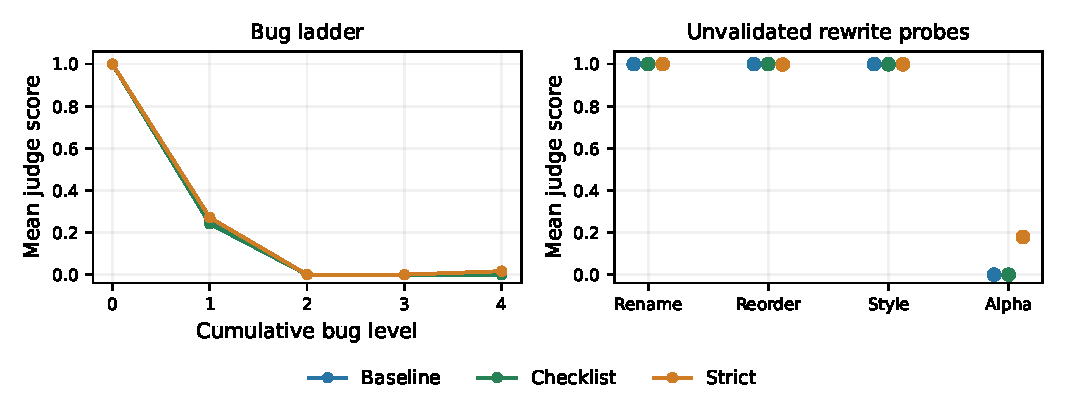
\includegraphics[width=\linewidth]{figures/codex_property_checks.pdf}
\caption{\textbf{Early bug edits and malformed alpha probes lower the Codex judges' mean scores.} Each point averages median scores over 24 problems, with three calls per problem and prompt; these are descriptive means, not uncertainty intervals.
Local reversals remain visible in Table~\ref{tab:codex_configs}.}
\label{fig:judge_sanity_checks}
\end{figure}

\subsection{The index tracks judge-level human agreement on the validation set}\label{sec:tivar_cross_model_results}\label{sec:validation-human-alignment}
% Provenance: experiments/archive/41_.../REPORT.md gate G0 (reproduces 0.833 / 0.905 / 0.738 and the Opus and Qwen rows to three decimals); experiments/archive/38_iclr_body_rewrite_to_trust_artifact_abstract/analysis/results/judge_level_diagnostics.csv.
The three primary families are GPT-5.3-Codex, Claude Opus 4.7, and Qwen3-Coder.
Each eight-configuration panel contains three semantic prompts, a deliberately lexical prompt on the same model, two GPT-4o-mini prompts, edit distance, and a random control.
These are family panels with shared controls, not eight independent models per family.
Scores are medians over three repeated calls for language-model judges; the Codex-panel controls use nine repeats, and the other panels use three.
Figure~\ref{fig:tivar_cross_model_avg} uses the fixed equal-weight index of Equation~\ref{eq:tivar}, normalized within each family panel.
Its judge-level Spearman association is positive for each primary family and rating view (Table~\ref{tab:tivar_cross_model_results}).
For Codex, the averaged-rating Pearson and Kendall associations are $0.868$ and $0.643$.
Exact permutation probabilities over all $8!$ orderings are $0.096$, $0.022$, and $0.132$ for Claude Opus and $0.005$, $0.243$, and $0.011$ for Qwen3-Coder on averaged, pass1, and pass2 ratings (Appendix~\ref{app:judge-level-diagnostics}).
Only some cells are individually distinguishable from a random ordering at the $0.05$ level, and the nine tests are unadjusted.
Excluding random, edit distance, and the lexical prompt leaves five semantic configurations, with averaged-rating associations of $0.900$ for Codex, $0.600$ for Claude Opus, and $0.900$ for Qwen3-Coder.
A separate Leanstral panel has averaged-rating association $-0.095$ (Appendix~\ref{app:negative-results}), so the positive result did not hold for every recorded family even on this panel.
On the held-out judges of Section~\ref{sec:transfer}, the same index normalized on the train configurations has association $-0.332$.

\begin{figure}[htbp]
\centering
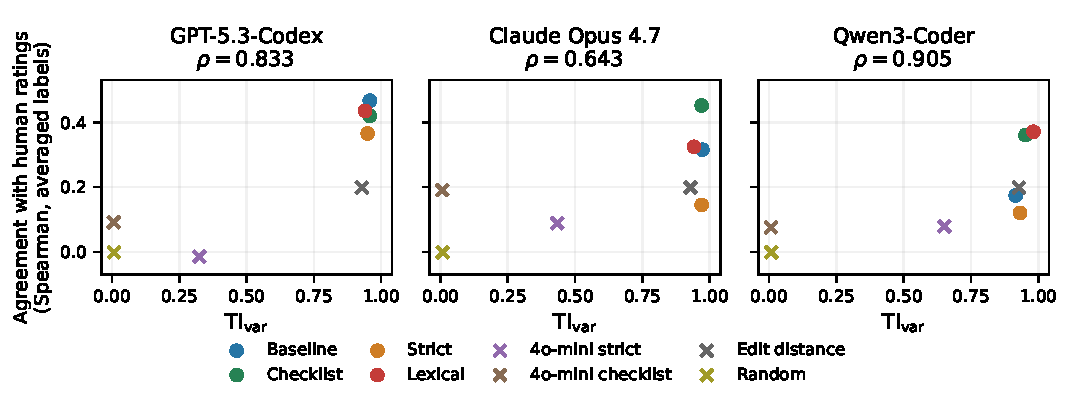
\includegraphics[width=\linewidth]{figures/judge_agreement_fixed_index.pdf}
\caption{\textbf{On the validation set the fixed equal-weight index has a positive association with human agreement in each primary family, but high index values do not rule out lexical judges.} Each point is one configuration; the vertical axis is its Spearman agreement with averaged human ratings on 72 pairs.
Panel titles report the correlation across eight configurations; Table~\ref{tab:tivar_cross_model_results} gives Codex uncertainty.}
\label{fig:tivar_cross_model_avg}
\end{figure}

\begin{table}[htbp]
\centering\small
\begin{tabular}{@{}lrrrrrr@{}}
\toprule
& \multicolumn{4}{c}{Averaged ratings} & \multicolumn{2}{c}{$\mathrm{TI}_{\mathrm{var}}$ by pass} \\
\cmidrule(lr){2-5}\cmidrule(lr){6-7}
Family & $v1$ & $v2$ & $\mathrm{GM}_{.4,.6}$ & $\mathrm{TI}_{\mathrm{var}}$ & pass1 & pass2 \\
\midrule
Codex & 0.762 & 0.476 & 0.857 & 0.833 & 0.905 & 0.738 \\
Claude Opus & 0.429 & 0.143 & 0.714 & 0.643 & 0.810 & 0.595 \\
Qwen3-Coder & 0.524 & 0.500 & 0.786 & 0.905 & 0.476 & 0.857 \\
\midrule
\multicolumn{4}{l}{Codex $\mathrm{TI}_{\mathrm{var}}$: 95\% interval} & $[0.24,1.00]$ & $[0.41,1.00]$ & $[0.11,1.00]$ \\
\multicolumn{4}{l}{Codex $\mathrm{TI}_{\mathrm{var}}$: permutation $p$} & 0.017 & 0.005 & 0.045 \\
\bottomrule
\end{tabular}
\caption{\textbf{On the validation set the fixed index is competitive with a two-component geometric comparison whose weights were selected on pass1.} Entries are Spearman correlations between each index and judge-level human agreement, with eight configurations per family.
Codex intervals and permutation probabilities use 10{,}000 resamples and permutations, seed 42; exact permutation probabilities for every cell are in Appendix~\ref{app:judge-level-diagnostics}.
Appendix~\ref{app:index-definitions} defines all indices.}
\label{tab:tivar_cross_model_results}\label{tab:cross_model_index_compare_avg}
\end{table}

\subsection{Human agreement alone can miss a bad judge}\label{sec:lexical-judge}
The lexical prompt, \texttt{BAD\_STRINGY}, instructs the model to ignore theorem meaning and grade textual overlap.
On the Codex panel, its human agreement of $0.435$ lies among the semantic prompts' values, $0.365$--$0.466$.
A validation protocol that stops at human agreement would accept it.
Yet it reverses on 20 of 24 bug ladders (Table~\ref{tab:codex_configs}).
The scalar does not expose it either: its index value is $0.940$, below the three semantic prompts but far above the failing GPT-4o-mini configurations, and edit distance scores $0.928$.
In the Qwen panel, the lexical configuration even has the highest index value, $0.982$.
The failure report therefore carries information that both human agreement and the scalar can miss, which is why the transfer study keeps the per-component report beside any index.
The same prompt is the lexical configuration of the transfer study, where it anchors the low end of both axes in Figure~\ref{fig:transfer}.

\begin{table}[htbp]
\centering\small
\begin{tabular}{@{}lrrr@{}}
\toprule
Codex-panel configuration & Human $\rho$ (avg) & $\mathrm{TI}_{\mathrm{var}}$ & Ladders with reversals \\
\midrule
Baseline prompt & 0.466 & 0.958 & 0/24 \\
Checklist prompt & 0.419 & 0.958 & 0/24 \\
Strict prompt & 0.365 & 0.950 & 4/24 \\
Lexical prompt & 0.435 & 0.940 & 20/24 \\
GPT-4o-mini, strict & $-0.014$ & 0.324 & 18/24 \\
GPT-4o-mini, checklist & 0.092 & 0.007 & 16/24 \\
Edit distance & 0.199 & 0.928 & 24/24 \\
Random & $-0.001$ & 0.008 & 24/24 \\
\bottomrule
\end{tabular}
\caption{\textbf{The lexical judge agrees with the rater despite frequent bug-ladder reversals, and the scalar index penalizes it only slightly.} A reversal is any local score increase as cumulative edits are added; the diagnostic uses the recorded repeat-aggregated scores.}
\label{tab:codex_configs}
\end{table}

\paragraph{Choice of index, sensitivity, and diagnostics.}
The two-component geometric comparison in Table~\ref{tab:tivar_cross_model_results} uses bug monotonicity and decision stability with weights $0.4$ and $0.6$ selected on pass1, and is numerically higher than $\mathrm{TI}_{\mathrm{var}}$ for Codex and Opus on averaged ratings.
The bug-monotonicity component alone has averaged-rating associations of $0.643$, $0.467$, and $0.690$, and the full index has higher point correlations in eight of nine family--pass cells, a descriptive comparison on reused ratings (Appendix~\ref{app:judge-level-diagnostics}).
A separate search over six component weights gives cross-pass associations of $0.810$ and $0.786$, and the pass1-selected geometric form reaches $0.769$ with a 95\% interval of $[0.34,0.95]$ on an expanded 13-configuration panel (Appendices~\ref{app:moved-results} and~\ref{app:expanded-panel}); neither is a held-out estimate.
Recomputing the fixed index on a local grid of weight triples gives averaged-rating ranges of $0.738$--$0.857$ for Codex, $0.643$--$0.714$ for Opus, and $0.881$--$0.976$ for Qwen (Appendix~\ref{app:weight-sensitivity}).
Among the recorded diagnostics, weak monotonicity on bug ladders has the largest association with human agreement on each rating view (Table~\ref{tab:property_assoc}); the archived field name \texttt{P3\_weak\_mono} refers to this bug statistic, not to a deletion property.
A historical sweep of the artifact-score threshold from $0.60$ to $0.85$ lowers the decision-flip rate from $0.058$ to $0.046$ with overlapping intervals (Table~\ref{tab:exp13_threshold_sweep}); it thresholds $J_\theta(x,g)$, not the judge-level index.

\begin{table}[htbp]
\centering\small
\begin{tabular}{@{}lrrr@{}}
\toprule
Measured diagnostic & pass1 & pass2 & avg \\
\midrule
Mean identity-rewrite score & $-0.21$ (0.62) & 0.02 (0.98) & $-0.02$ (0.98) \\
Bug-rank monotonicity & 0.60 (0.13) & 0.67 (0.08) & 0.71 (0.06) \\
Bug weak monotonicity & 0.63 (0.11) & 0.78 (0.03) & 0.75 (0.04) \\
Repeat decision stability & 0.47 (0.24) & $-0.23$ (0.57) & 0.14 (0.76) \\
\bottomrule
\end{tabular}
\caption{\textbf{Bug weak monotonicity has the largest observed association among the measured diagnostics of the validation set; this table contains no deletion-ladder result.} Entries are Spearman correlations with human agreement across eight Codex-panel configurations; unadjusted permutation probabilities appear in parentheses.}
\label{tab:property_assoc}
\end{table}

\subsection{Provenance of the validation set}\label{app:provenance}
% Provenance: experiments/archive/41_paper_panel_provenance_audit_and_vb_expert_label_rescore/REPORT.md (label identity 75/75 and 72/75; task classification 1 / 7 / 17; views V1 and V3 with task-clustered bootstrap, 10,000 resamples, seed 42, exact permutation over 8! orderings).
A zero-call audit traced the panel's ratings and reference files after the earlier version was written.
The two rating passes are byte-identical, on the shared items, to the superseded old-prompt rating passes of \textsc{VeriBench}'s first participant (75 of 75 and 72 of 75 items), whom \textsc{VeriBench} later re-rated under a corrected prompt together with four more experts; the names of the two passes are swapped relative to the order in which they were rated.
The frozen judge pipeline resolved gold files from a copy of \textsc{VeriBench} frozen on 2026-04-12, before the rating window opened, and silently skipped the one task whose gold filename had changed.
Of the 24 tasks it scored, only seven have reference bytes identical to what the rater saw at the time the ratings were committed; the other 17 references were rewritten in between.
Re-scoring the association on the 21 matched items from those seven tasks against \textsc{VeriBench}'s corrected three-expert mean gives $0.333$ $[-0.321, 0.543]$ for Codex, $-0.381$ $[-0.524, 0.657]$ for Claude Opus, and $0.667$ $[-0.575, 0.898]$ for Qwen3-Coder, with exact permutation probabilities of $0.428$, $0.360$, and $0.083$ over eight configurations.
Under the audit's pre-registered rule, which required one sign in all three families, this is inconclusive; every interval crosses zero, and the matched-item association is not stable to dropping a single configuration.
The panel's numbers therefore stand as recorded on the ratings and references the judges saw, with the caveat that those references were not the ones the rater rated for most tasks.

\subsection{Selection bias from reusing the validation set}\label{app:selection-bias}
% Provenance: experiments/archive/40_best_of_k_judge_selection_bias_validation_set/REPORT.md (analyses A--D; 109 configurations; 4,000 draws; Monte Carlo standard error of each mean overstatement 0.004--0.005); figure copied from its figures/best_of_k_selection_bias.pdf.
We measured how much choosing among judge configurations on the 72 validation pairs overstates the winner's agreement, using only recorded scores.
The pool contains the 109 distinct configurations scored on exactly these pairs, excluding random and edit-distance controls.
When ratings are permuted in whole-problem blocks, the best of eight configurations still reaches a mean Spearman agreement of $0.150$ (95th percentile $0.317$), and the best of all 109 reaches $0.263$ (Figure~\ref{fig:selection-bias}a).
The observed agreement of 31 configurations exceeds $0.399$, the 95th percentile of the maximum over all 109, so the strongest agreements are not selection artifacts.
Chosen on 12 problems, the best of eight overstates its agreement on the other 12 problems by $0.153$ on averaged ratings, $0.117$ on pass1, and $0.194$ on pass2, averaged over 4{,}000 random splits with a Monte Carlo standard error of at most $0.005$; individual splits range from $-0.334$ to $+0.689$ (Figure~\ref{fig:selection-bias}b--c).
Beyond eight candidates, choosing among more configurations lowers the held-out agreement of the choice, from $0.335$ to $0.296$ at 109.
A latent-quality simulation fitted to the panel's inter-pass agreement and clustering reproduces the half-panel overstatement within $0.02$ and places it at about $0.10$ for eight candidates chosen on all 72 pairs.
Choosing by a label-free index never overstates agreement by more than $0.01$, but its held-out agreement is close to that of a random choice ($0.23$--$0.30$ against $0.27$--$0.28$ for two to 32 candidates).
At the judge level, taking the maximum over the four reported index forms multiplies the exact two-sided permutation probabilities by $1.9$ to $3.2$; four of nine family--rating cells remain below $0.05$, against six unadjusted.
These measurements motivated the split over judge models in Section~\ref{sec:property-protocol}: selection and evaluation must use different judges, and a label-free selector must be shown to pick better judges than chance before it can replace ratings.

\begin{figure}[htbp]
\centering
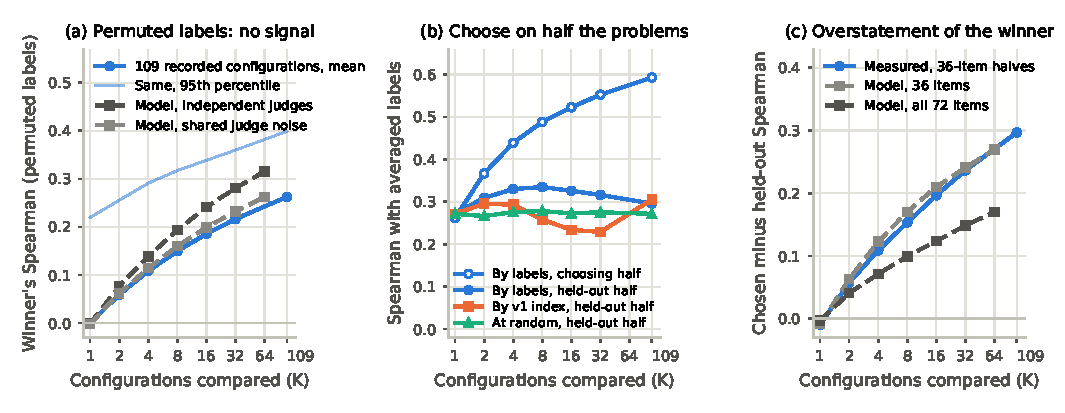
\includegraphics[width=\linewidth]{figures/best_of_k_selection_bias.pdf}
\caption{\textbf{Choosing among configurations on the validation ratings overstates the winner's agreement.} (a) Largest agreement among $K$ configurations with block-permuted ratings.
(b) Agreement of the configuration chosen on 12 problems, on those problems and on the other 12.
(c) Chosen-minus-held-out agreement, measured on half panels and simulated for half and full panels; means over 4{,}000 draws.}
\label{fig:selection-bias}
\end{figure}
